
\documentclass[11pt,t]{beamer}
\usetheme[sedes]{kuleuven_new_bottom_classic}	%OPTIONS for TITLE PAGE: normal (default), sedes

%%% OTHER SETTINGS
\usefonttheme[onlymath]{serif}	     % math font with serifs, delete to make it sans-serif
\setbeamertemplate{footline}[body]   % delete this line to remove footline bar on all frames
\usepackage[orientation=landscape,size=custom,width=16,height=9,scale=0.5,debug]{beamerposter} %enable for widescreen 16:9 ratio

%%% ADDED PACKAGES:
\usepackage[english]{babel}
\usepackage{amsfonts}
\usepackage{amssymb}
\usepackage{colortbl}
\usepackage{natbib}  
\usetikzlibrary{calc}
 
\hypersetup{%
       citecolor=kul-blue
}

%----------------------------------------------------

\title{Earth and Environmental Sciences:\\Open Data, Open Source Code}
\author{Prof. dr. ir. Gabri\"elle De Lannoy}
\institute{KU Leuven - Faculty Bioscience Engineering}
\date{6 May 2026}

\begin{document}

%\maketitle

%% Title page
\begin{frame}[plain,noframenumbering]
	\titlepage
\end{frame}

    
%========================================================
\section{Open Research}
%========================================================

\begin{frame}{Research Topics}
\begin{itemize}
    \item enter your ideas
    \item and so on
\end{itemize}
\end{frame}

%========================================================
\section{Open Data}
%========================================================

\begin{frame}{Satellite Data}

\vspace{-0.2cm}
\begin{columns}[t]
\begin{column}[T]{0.49\linewidth}
	\begin{block}{Satellite data are a public good}
    \begin{itemize}
		\item For everyone
        \item
    \end{itemize}
	\end{block}
\end{column}
\begin{column}[T]{.49\textwidth}
\begin{alertblock}{Anything bad?} %creators and consumers
	   \begin{itemize}
		\item Maintenance, misinterpretation
        \item 
	   \end{itemize}
	\end{alertblock}
\end{column}
\end{columns}

\end{frame}

%========================================================
\section{Open Source Code}
%========================================================

\begin{frame}{AquaCrop Model}

\centering
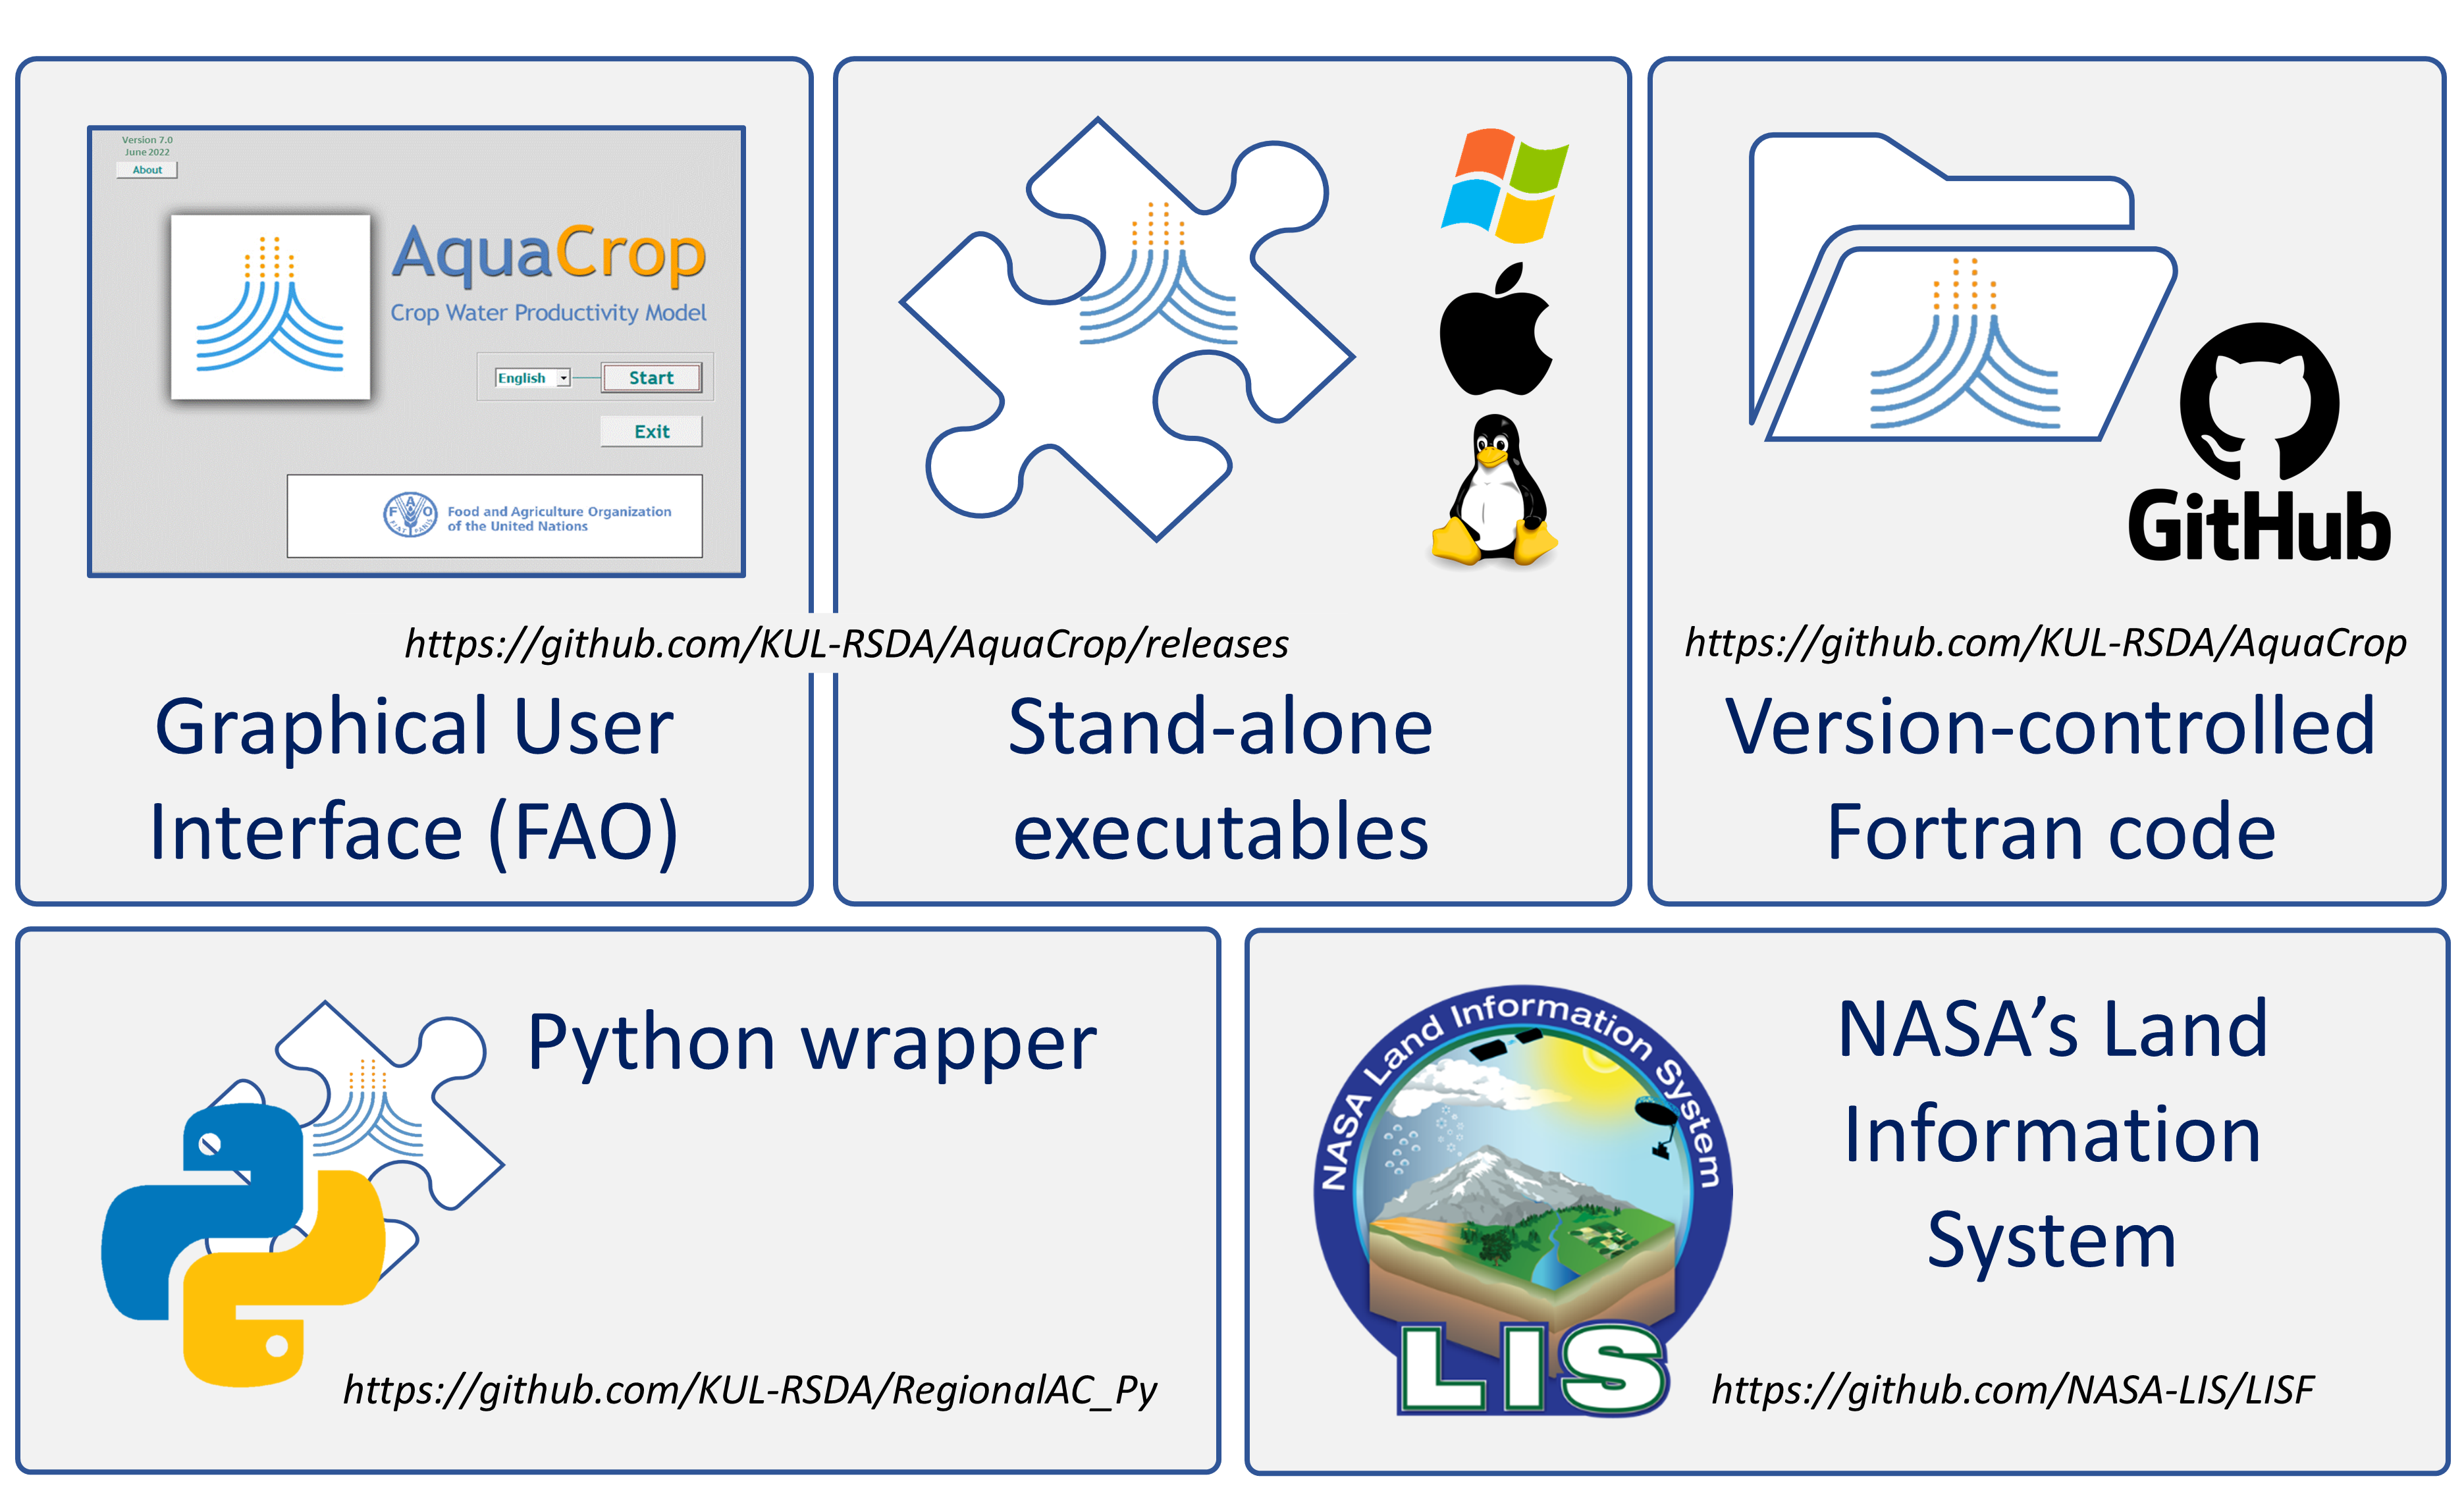
\includegraphics[trim=0cm 0cm 0cm 0cm,clip,width=0.65\linewidth]{Figures/Fig1.png}\\ \vspace{-0.3cm}
 {\it{\tiny{\citep{DeLannoyetal26}}}}

\end{frame}


%========================================================
\section{Data Assimilation / Machine Learning}
%========================================================

\begin{frame}{Data Assimilation}

\centering{\bf\it{"The whole is greater than the sum of the parts" (Aristotle)}\\ {\it{\tiny{\citep{DeLannoyetal22}}}}}

\end{frame}

%========================================================
\section*{Conclusions}
%========================================================

\begin{frame}{Conclusions}

\vspace{1cm}
\begin{block}{Serve the world}
\begin{itemize}
    \item science is a global public good
	\item {\color{kul-blue}{open satellite data}}
	\item {\color{kul-blue}{open source code}}
	\item {\color{kul-blue}{open access}}
	\item give and take
\end{itemize}
\end{block}

\end{frame}

%========================================================
\section*{References}
%========================================================
\begin{frame}[allowframebreaks,noframenumbering,fragile]{Some references}

\bibliographystyle{apa-good} %{copernicus} %emsla} %plain} %emsla}
{\tiny{\bibliography{references}}}

\end{frame}


\end{document}
\endinput

